\section{Introduction}


\begin{frame}{A little history.}
	When it comes to degree sequences, there are a few familiar faces in the history of the study.
		\begin{itemize}
			\item Havel and Hakimi explored degree sequences for graphs in the 1960s.
			\item In 1994, we got a paper from Gary Chartrand, Heather Gavlas, Frank Harary, and Michelle Schultz detailing initial findings.
			\item In 1996 the paper discussed today was published Jing-Ho Yan, Ko-Wei Lih, David Kuo, and Gerard. G Chang.
		\end{itemize}
\end{frame}

\begin{frame}
	\begin{figure}
		\centering 
		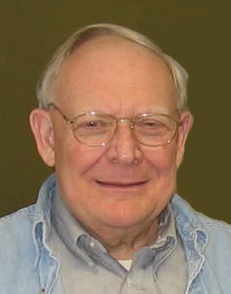
\includegraphics{GaryChartrand.png}
		\caption[]{Gary Chartrand}
	\end{figure}
\end{frame}



\section{Definitions}
\begin{frame}
    \begin{definition}
        A \textit{signed} graph is a graph where each edge is labelled as \textit{positive} ($+$) or \textit{negative} ($-$).
    \end{definition}
    \begin{figure}[H]
        \centering
        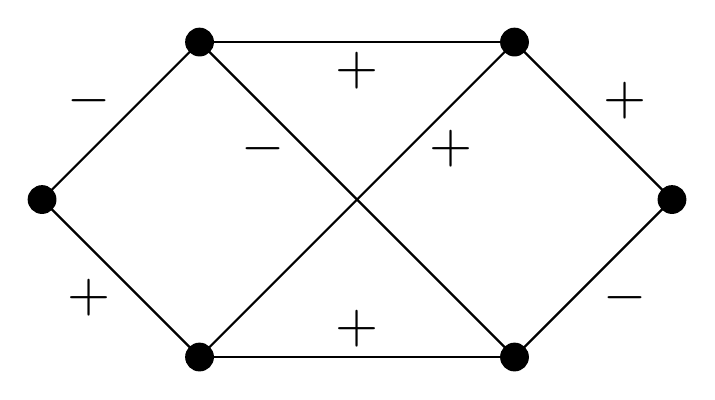
\begin{tikzpicture}[scale=1]
            %graph
            \draw[thick] (2,2)--(4,0);

            \node[right] at (3,1.25) {\(\scalebox{2}{\(+\)}\)};
    
            \draw[thick] (4,0)--(2,-2);

            \node[right] at (3,-1.25) {\(\scalebox{2}{\(-\)}\)};
    
            \draw[thick] (2,-2)--(-2,-2);

            \node[above] at (0,-2) {\(\scalebox{2}{\(+\)}\)};
    
            \draw[thick] (-2,-2)--(-4,0);

            \node[left] at (-3,-1.25) {\(\scalebox{2}{\(+\)}\)};
    
            \draw[thick] (-4,0)--(-2,2);

            \node[left] at (-3,1.25) {\(\scalebox{2}{\(-\)}\)};
    
            \draw[thick] (-2,2)--(2,2);

            \node[below] at (0,2) {\(\scalebox{2}{\(+\)}\)};
    
            \draw[thick] (-2,2)--(2,-2);

            \node[below] at (1.2,1) {\(\scalebox{2}{\(+\)}\)};
    
            \draw[thick] (2,2)--(-2,-2);

            \node[below] at (-1.2,1) {\(\scalebox{2}{\(-\)}\)};
    
            \draw[fill] (-2,2) circle (5pt);
    
            \draw[fill] (2,2) circle (5pt);
    
            \draw[fill] (4,0) circle (5pt);
    
            \draw[fill] (2,-2) circle (5pt);
    
            \draw[fill] (-2,-2) circle (5pt);
    
            \draw[fill] (-4,0) circle (5pt);
        \end{tikzpicture}
    \end{figure}
\end{frame}

\begin{frame}
    If an edge $uv$ is labelled with a $+$, we denote the edge by $uv^{+}$.
    \begin{definition}
        For any vertex $u \in V(G)$
        \begin{enumerate}
            \item The \textit{positive} degree of the vertex is
            \begin{equation*}
                d^{+}(u) = |\{v \in V(G) \mid uv^+ \in E(G)\}|
            \end{equation*}
            \item The \textit{negative} degree of the vertex is
            \begin{equation*}
                d^{-}(u) = |\{v \in V(G) \mid uv^- \in E(G)\}|
            \end{equation*}
            \item The \textit{signed} degree of a vertex is
            \begin{equation*}
                sd(u) = d^+(u) - d^-(u)
            \end{equation*}
        \end{enumerate}
    \end{definition}
\end{frame}

\begin{frame}
    \begin{figure}[H]
        \centering
        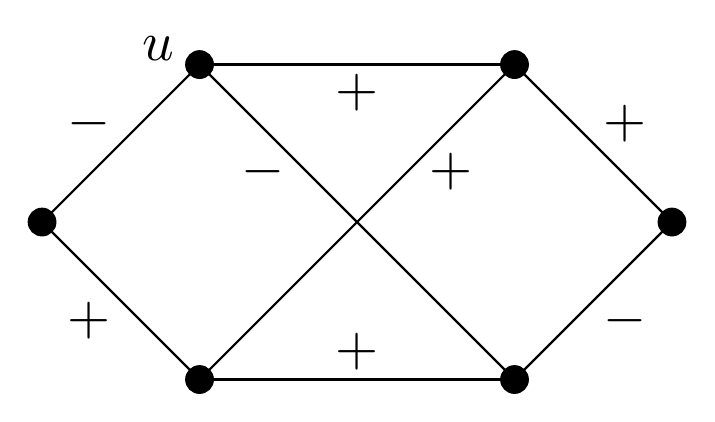
\begin{tikzpicture}[scale=1]
            %graph
            \draw[thick] (2,2)--(4,0);

            \node[right] at (3,1.25) {\(\scalebox{2}{\(+\)}\)};
    
            \draw[thick] (4,0)--(2,-2);

            \node[right] at (3,-1.25) {\(\scalebox{2}{\(-\)}\)};
    
            \draw[thick] (2,-2)--(-2,-2);

            \node[above] at (0,-2) {\(\scalebox{2}{\(+\)}\)};
    
            \draw[thick] (-2,-2)--(-4,0);

            \node[left] at (-3,-1.25) {\(\scalebox{2}{\(+\)}\)};
    
            \draw[thick] (-4,0)--(-2,2);

            \node[left] at (-3,1.25) {\(\scalebox{2}{\(-\)}\)};
    
            \draw[thick] (-2,2)--(2,2);

            \node[below] at (0,2) {\(\scalebox{2}{\(+\)}\)};
    
            \draw[thick] (-2,2)--(2,-2);

            \node[below] at (1.2,1) {\(\scalebox{2}{\(+\)}\)};
    
            \draw[thick] (2,2)--(-2,-2);

            \node[below] at (-1.2,1) {\(\scalebox{2}{\(-\)}\)};
    
            \draw[fill] (-2,2) circle (5pt);

            \node[left] at (-2.2,2.2) {\(\scalebox{2}{\(u\)}\)};
    
            \draw[fill] (2,2) circle (5pt);
    
            \draw[fill] (4,0) circle (5pt);
    
            \draw[fill] (2,-2) circle (5pt);
    
            \draw[fill] (-2,-2) circle (5pt);
    
            \draw[fill] (-4,0) circle (5pt);
        \end{tikzpicture}
    \end{figure}
    \begin{align*}
        d^+(u) = 1 && d^-(u) = 2 && sd(u) = -1 && d(u) = 3
    \end{align*}
\end{frame}

\begin{frame}
    \begin{definition}
        A \textit{signed} degree sequence is a finite list of integers
        \begin{equation*}
            \sigma : d_1, d_2, \dots, d_n
        \end{equation*}
        The sequence is \textbf{s-graphical} if there exists a signed graph $(V,E)$ with vertices $V = \{v_1,\dots,v_n\}$ such that $d_i = sd(v_i)$.
    \end{definition}
    In our example from before, the signed degree sequence would be
    \begin{equation*}
        \sigma : -1, 3, 0, -1, 3, 0
    \end{equation*}
\end{frame}
